% RESULTS

\subsection{Identification of the \textit{in vivo} WASH complex proteome}

While multiple mutations within the WASH complex have been identified in humans 
(Assoum et al., 2020; Elliott et al., 2013; Ropers et al., 2011; 
Valdmanis et al., 2007), how these mutations lead to neurological
dysfunction remains unknown \textbf{(Figure 1A)}. Given that previous work in
non-neuronal cultured cells and non-mammalian organisms have established that
the WASH complex functions in endosomal trafficking, we first aimed to determine
whether this role was conserved in the mouse nervous system (Alekhina et al.,
2017; Billadeau et al., 2010; Derivery et al., 2009; Gomez et al., 2012; Gomez
and Billadeau, 2009). To discover the likely molecular functions of the neuronal
WASH complex, we utilized an in vivo BioID (iBioID) paradigm developed in our
laboratory to identify the WASH complex proteome from brain tissue (Uezu et al.,
2016). BioID probes were generated by fusing a component of the WASH complex,
WASH1 (gene: Washc1), with the promiscuous biotin ligase, BioID2 (WASH1-BioID2,
Figure 1B), or by expressing BioID2 alone (negative control, solubleBioID2)
under the neuron-specific, human Synapsin-1 promoter (Kim et al., 2016). We
injected adenoviruses (AAV) expressing these constructs into the cortex of
wild-type postnatal day zero (P0) mice \textbf{(Figure 1B)}. Two weeks post-injection, we
administered daily subcutaneous biotin for seven days to biotinylate in vivo
substrates. The viruses displayed efficient expression and activity in brain
tissue, as evidenced by colocalization of the WASH1-BioID2 viral epitope (HA)
and biotinylated proteins (Streptavidin) \textbf{(Figures 1C-F)}. For label-free
quantitative high-mass accuracy LC-MS/MS analyses, whole brain samples were
collected at P22, snap-frozen, and processed as previously described (Uezu et
al., 2016). A total of 2,311 proteins were identified across all three
experimental replicates, which were further analyzed for those with significant
enrichment in WASH1-BioID2 samples over solubleBioID2 negative controls 
\textbf{(Table S1)}. 

% Figure 1.
%\begin{figure}
%\begin{fullwidth}
%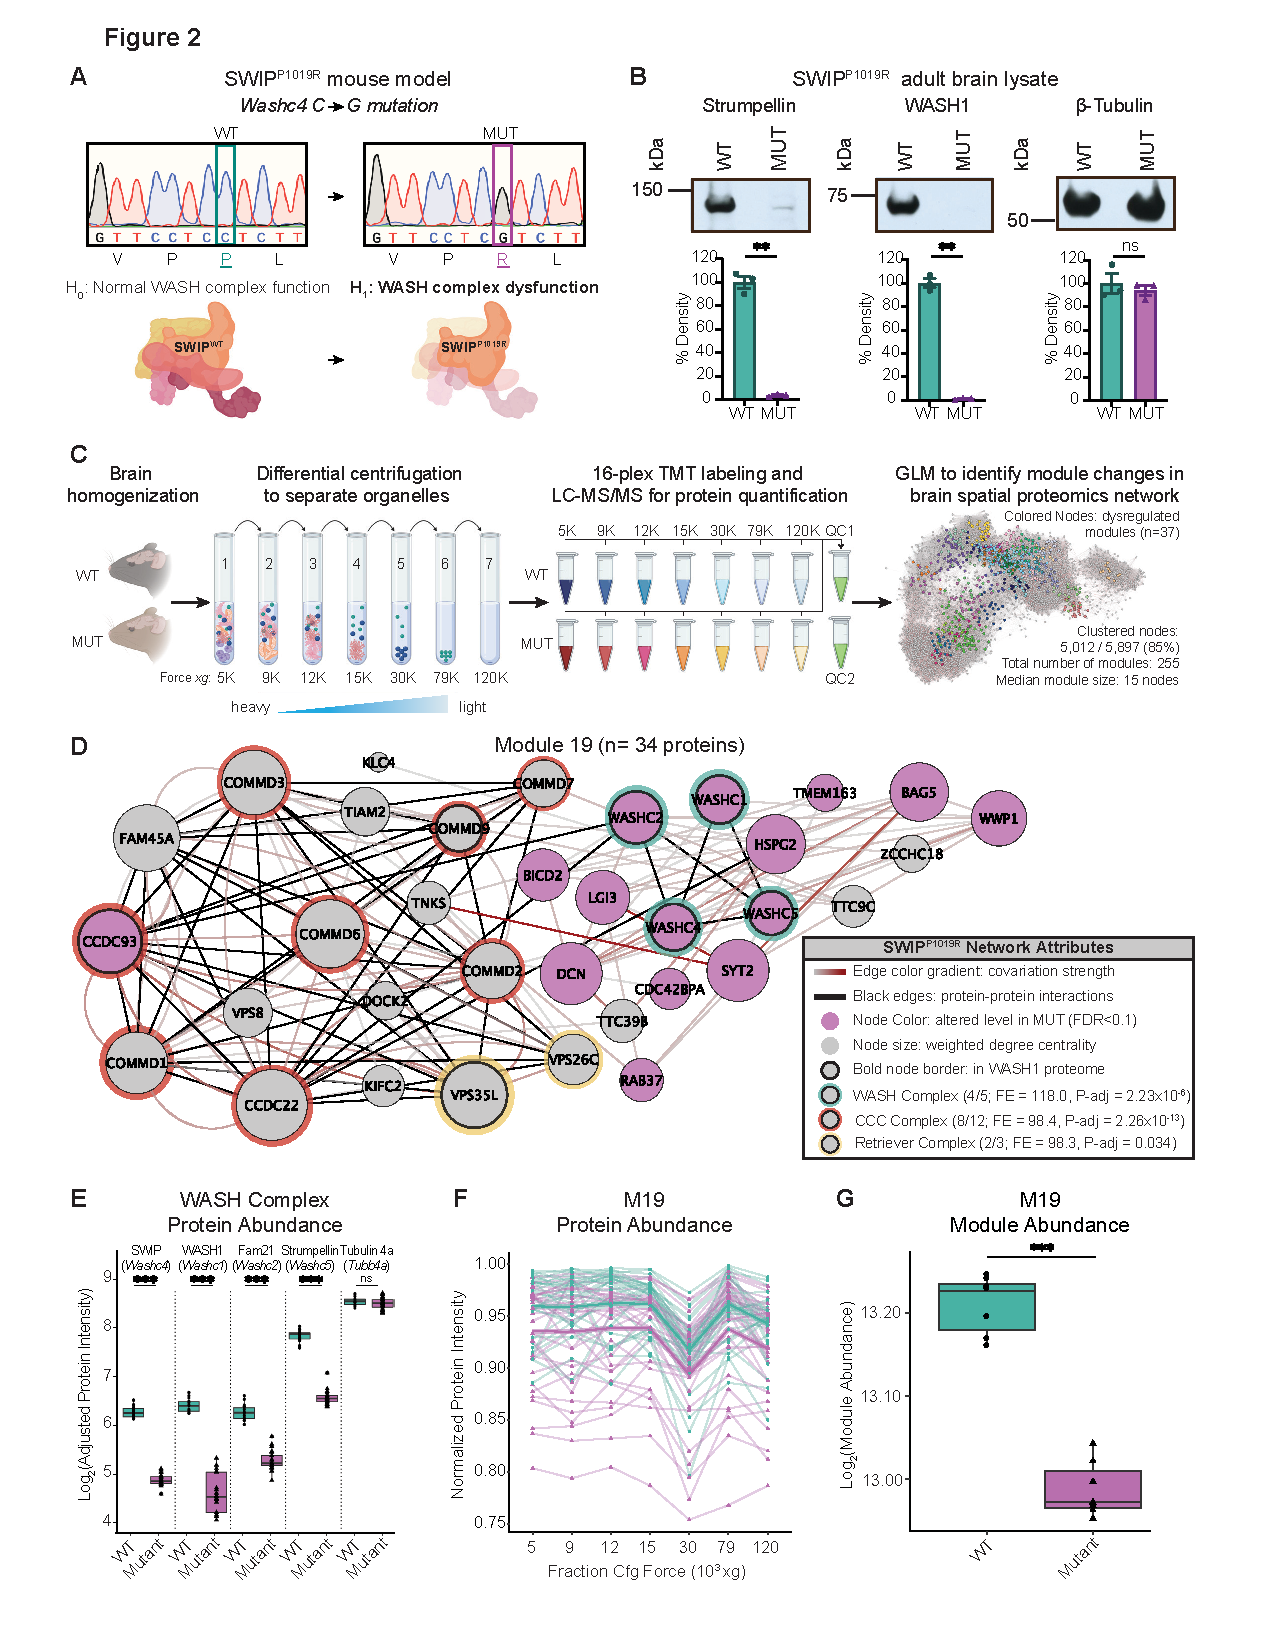
\includegraphics[height=0.95\linewidth, keepaspectratio]{Figure_01}
%	\caption{This is a caption.}
%\label{fig:fullwidth}
%\end{fullwidth}
%\end{figure}

The resulting neuronal WASH proteome included 174 proteins that were
significantly enriched (Fold-change $\geq$ 3.0, Benjamini-Hochberg P-Adjust $<$ 0.1,
\textbf{Figure 1G}). Of these proteins, we identified all five WASH complex components
\textbf{(Figure 1H)}, as well as 13 previously reported WASH complex interactors 
\textbf{(Figure 1I)} (McNally et al., 2017; Phillips-Krawczak et al., 2015; Simonetti and
Cullen, 2019; Singla et al., 2019), which provided strong validity for our
proteomic approach and analyses. Additional bioinformatic analyses of the
neuronal WASH proteome identified a network of proteins implicated in vesicular
trafficking, including 23 proteins enriched for endosomal functions \textbf{(Figure 1J)}
and 24 proteins enriched for endocytic functions \textbf{(Figure 1K)}. Among these
endosomal and endocytic proteins were components of the recently identified
endosomal sorting complexes, CCC (CCDC93 and COMMD9) and Retriever (VPS35L)
(Phillips-Krawczak et al., 2015; Singla et al., 2019), as well as multiple
sorting nexins important for recruitment of trafficking regulators to the
endosome and cargo selection, such as SNX1-3, and SNX16 (Kvainickas et al.,
2017; Maruzs et al., 2015; Simonetti et al., 2017). These data demonstrated that
the WASH complex interacts with many of the same proteins in neurons as it does
in yeast, amoebae, flies, and mammalian cell lines. Furthermore, there were 32
proteins enriched for cytoskeletal regulatory functions \textbf{(Figure 1L)}, including
actin-modulatory molecules such as the Arp2/3 complex subunit ARPC5, which is
consistent with WASH’s role in activating this complex to stimulate actin
polymerization at endosomes for vesicular scission (Billadeau et al., 2010;
Derivery et al., 2009). The WASH1-BioID2 isolated complex also contained 28
proteins known to localize to the excitatory post-synapse \textbf{(Figure 1M)}. This
included many core synaptic scaffolding proteins, such as SHANK2-3 and DLGAP2-4
(Chen et al., 2011; Mao et al., 2015; Monteiro and Feng, 2017; Wan et al.,
2011), as well as modulators of synaptic receptors such as SYNGAP1 and SHISA6
(Barnett et al., 2006; Clement et al., 2012; Kim et al., 2003; Klaassen et al.,
2016), which was consistent with the idea that vesicular trafficking plays an
important part in synaptic function and regulation. Taken together, these
results support a major endosomal trafficking role of the WASH complex in mouse
brain. 

\subsection{The SWIP\textsuperscript{P1019R} mutation destabilizes the WASH complex}

To determine how disruption of the WASH complex may lead to
disease, we generated a mouse model of a human missense mutation found in
children with intellectual disability, WASHC4\textsuperscript{c.3056c>g} 
(protein: SWIP\textsuperscript{P1019R}) (Ropers et al., 2011). 
Due to the sequence homology of human and mouse Washc4
genes, we were able to introduce the same point mutation in exon 29 of murine
Washc4 using CRISPR (Derivery and Gautreau, 2010; Ropers et al., 2011). This C>G
point mutation results in a Proline>Arginine substitution at position 1019 of
SWIP’s amino acid sequence \textbf{(Figure 2A)}, a region thought to be critical for its
binding to the WASH component, Strumpellin (Jia et al., 2010; Ropers et al.,
2011). Western blot analysis of brain lysate from adult homozygous SWIP\textsuperscript{P1019R}
mutant mice (referred to from here on as MUT mice) displayed significantly
decreased abundance of two WASH complex members, Strumpellin and WASH1 
\textbf{(Figure 2B)}. These results phenocopied data from the human patients (Ropers et al.,
2011) and suggested that the WASH complex is unstable in the presence of this
SWIP point mutation in vivo. To test whether this mutation disrupted
interactions between WASH complex subunits, we compared the ability of wild-type
SWIP (WT) and SWIP\textsuperscript{P1019R} (MUT) to co-immunoprecipitate with Strumpellin and
WASH1 in HEK cells. Compared to WT, MUT SWIP co-immunoprecipitated significantly
less Strumpellin and WASH1 (IP: 54.8\% and 41.4\% of WT SWIP, respectively),
suggesting that the SWIP\textsuperscript{P1019R} mutation hinders WASH complex formation 
\textbf{(Figure 2 and Figure Supplement 1)}. Together these data support the notion that 
SWIP\textsuperscript{P1019R} is a damaging mutation that not only impairs its function, 
but also results in significant reductions of the WASH complex as a whole.

\subsection{Spatial proteomics analysis of SWIP\textsuperscript{P1019R} mutant mouse brain}

Next, we aimed to understand the impact of the SWIP\textsuperscript{P1019R} mutation on the
subcellular organization of the mouse brain proteome. We performed spatial
proteomics by following the protocol established by Geladaki \textit{et al.}, with
modifications for homogenization of brain tissue (Geladaki et al., 2019; Hallett
et al., 2008). We isolated seven subcellular fractions from brain tissue and
quantified proteins in these samples using 16-plex TMT proteomics. Using this
spatial proteomics dataset, we developed a data-driven clustering approach to
classify proteins into subcellular compartments. This approach, which differs
from the support vector machine learning algorithm employed by Geladaki et al.
(2019), was motivated by the lack of a large corpus of brain-specific protein
subcellular localization information, and the greater complexity of brain tissue
compared to cultured cells. In addition to evaluating differential protein
abundance between WT and SWIP\textsuperscript{P1019R} MUT brain, we utilized this spatial
proteomics dataset to analyze network-level changes in groups of covarying
proteins to better understand WASH’s function and explore the cellular
mechanisms by which SWIP\textsuperscript{P1019R} causes disease. 

Brains from 10-month-old mice were gently homogenized to release intact
organelles, followed by successive centrifugation steps to enrich subcellular
compartments into different fractions based on their density \textbf{(Figure 2C)}
(Geladaki et al., 2019). Seven WT and seven MUT fractions (each prepared from
one brain, 14 samples total) were labeled with unique isobaric tandem-mass tags
and concatenated. We also included two sample pooled quality controls (SPQCs),
which allowed us to assess experimental variability and perform normalization
between experiments. By performing this experiment in triplicate, deep coverage
of the mouse brain proteome was obtained—across all 48 samples we quantified
86,551 peptides, corresponding to 7,488 proteins. After data pre-processing,
normalization, and filtering we retained 5,897 reproducibly quantified proteins
in the final dataset \textbf{(Table S2)}. 

We used generalized linear models (GLMs) to assess differential protein
abundance for intra-fraction comparisons between WT and MUT genotypes, and for
overall comparisons between WT and MUT groups, adjusted for baseline differences
in subcellular fraction. In the first analysis, there were 85 proteins with
significantly altered abundance in at least one of the 7 subcellular fractions
(Benjamini-Hochberg P-Adjust $<$ 0.1, \textbf{Table S2} and 
\textbf{Figure 2 Supplement 2}). Five proteins were differentially abundant 
between WT and MUT in all 7 fractions, including four WASH proteins 
and RAB21A—a known WASH interactor that functions in early endosomal 
trafficking (WASHC1, WASHC2, WASHC4, WASHC5, \textbf{Figure 2E}) 
(Del Olmo et al., 2019; Simpson et al., 2004). The abundance of the
remaining WASH complex protein, WASHC3, was found to be very low and was not
retained in the final dataset due to its sparse quantification. These data
affirm that the SWIP\textsuperscript{P1019R} mutation destabilizes the WASH complex. Next, to
evaluate global differences between WT and MUT brain, we analyzed the average
effect of genotype on protein abundance across all fractions. At this level,
there were 687 differentially abundant proteins between WT and MUT brain
(Bonferroni P-Adjust $<$ 0.05) \textbf{(Table S2)}. We then aimed to place these
differentially abundant proteins into a more meaningful biological context using
a systems-based approach.

For network-based analyses, we clustered the protein covariation network defined
by pairwise correlations between all 5,897 proteins. Our data-driven,
quality-based approach used Network Enhancement (Wang et al., 2018) to remove
biological noise from the covariation network and employed the Leiden algorithm
(Traag et al., 2019) to identify optimal partitions of the graph. We enforced
module quality by permutation testing (Ritchie et al., 2016) to ensure that
identified modules exhibited a non-random topology. Clustering of the protein
covariation graph identified 255 modules of proteins that strongly covaried
together (see Methods for complete description of clustering approach). 
To test for module-level differences between WT and MUT brain, we summarized
modules for each biological replicate (a single subcellular fraction prepared
from either a WT or MUT mouse) as the sum of their proteins, and extended our
GLM framework to identify changes in module abundance (adjusted for fraction
differences) between genotypes. 37 of the 255 modules exhibited significant
differences in WT versus MUT brain (Bonferroni P-Adjust $<$ 0.05; \textbf{Table S3}). 
Of note, the module containing the WASH complex, M19, was predicted to have
endosomal function by annotation of protein function, and was enriched for
proteins identified by WASH1-BioID2 (hypergeometric test P-Adjust $<$ 0.05, bold
node edges, \textbf{Figure 2D}). Similar to the WASH iBioID proteome \textbf{(Figure 1)}, M19
contained components of the CCC (CCDC22, CCDC93, COMMD1-3, COMMD6-7, and COMMD9)
and Retriever sorting complexes (VPS26C and VPS35L), but not the Retromer
sorting complex, suggesting that in the brain, the WASH complex may not interact
as closely with Retromer as it does in other cells \textbf{(Figure 2D)}. Across all
fractions, the abundance of M19 was significantly lower in MUT brain compared to
WT, providing evidence that the SWIP\textsuperscript{P1019R} mutation reduces the stability of
this protein subnetwork and impairs its function \textbf{(Figure 2F-G)}. 

In contrast to the decreased abundance of the WASH complex/endosome module, M19,
we observed three modules (M2, M159, and M213) which were enriched for lysosomal
protein components (Geladaki et al., 2019), and exhibited increased abundance in
MUT brain \textbf{(Figure 3)}. M159 \textbf{(Figure 3B)} contained the lysosomal protease
Cathepsin A (CTSA), while M213 \textbf{(Figure 3D)} contained Cathepsin B (CTSB), as well
as two key lysosomal hydrolases GLB1 and MAN2B2, and M2 \textbf{(Figure 3C)} contained
two Cathepsins (CTSS and CTSL) and several lysosomal hydrolases (e.g. GNS, GLA,
and MAN2B1) (Eng and Desnick, 1994; Mayor et al., 1993; Mok et al., 2003; Moon
et al., 2016; Patel et al., 2018; Regier and Tifft, 1993; Rosenbaum et al.,
2014). Notably, M2 also contained the lysosomal glycoprotein progranulin (GRN),
which is integral to proper lysosome function and whose loss is widely linked
with neurodegenerative pathologies (Baker et al., 2006; Pottier et al., 2016;
Tanaka et al., 2017; Zhou et al., 2018). In addition, M2 contained the hydrolase
IDS, whose loss causes a lysosomal storage disorder that can present with
neurological symptoms (Hopwood et al., 1993; Schröder et al., 1994). The overall
increase in abundance of modules M2, M159, and M213, and these key lysosomal
proteins (Figure 3E-G), may therefore reflect an increase in flux through
degradative lysosomal pathways in SWIP\textsuperscript{P1019R} brain. 

Furthermore, Module 2 \textbf{(Figure 3C)} included multiple membrane proteins and
extracellular proteins, such as ITGA5 (an integrin shown to be upregulated and
redistributed upon loss of WASH1), ATP13A2 (a cation transporter whose loss
causes a Parkinsonian syndrome), and MMP17 (an extracellular metalloprotease),
suggesting a link between these proteins and lysosomal enzymatic function
(English et al., 2000; Ramirez et al., 2006; Zech et al., 2011). Increased
abundance of these M2 proteins in MUT brain may indicate that WASH complex
disruption alters their cellular localization. Taken together, these changes
appear to reflect a pathological condition characterized by distorted lysosomal
metabolism and altered cellular trafficking.

In addition to these endo-lysosomal changes, network alterations were
evident for an endoplasmic reticulum (ER) module (M83), supporting a shift in
the proteostasis of mutant neurons \textbf{(Figure 2 and Figure Supplement 3B)}. Notably,
within the ER module, M83, there was increased abundance of chaperones (e.g.
HSPA5, PDIA3, PDIA4, PDIA6, and DNAJC3) that are commonly engaged in presence of
misfolded proteins (Bartels et al., 2019; Kim et al., 2020; Montibeller and de
Belleroche, 2018; Synofzik et al., 2014; Wang et al., 2016). This elevation of
ER stress modulators can be indicative of neurodegenerative states, in which the
unfolded protein response (UPR) is activated to resolve misfolded species
(Garcia-Huerta et al., 2016; Hetz and Saxena, 2017). These data demonstrate that
loss of WASH function not only alters endo-lysosomal trafficking, but also
causes increased stress on cellular homeostasis. 
Finally, besides these endo-lysosomal and homeostatic changes, we also observed
two synaptic modules (M35 and M248) that were reduced in MUT brain \textbf{(Figure
2 and Figure Supplement 3C-D)}. These included mostly excitatory post-synaptic
proteins such as HOMER2 and DLG4 (also identified in WASH1-BioID, \textbf{Figure 1}),
consistent with endosomal WASH influencing synaptic regulation. Decreased
abundance of these modules indicates that loss of the WASH complex may result in
failure of these proteins to be properly trafficked to the synapse.

\subsection{SWIP mutant neurons display endo-lysosomal structural abnormalities}

Combined, the proteomics data strongly suggested that endo-lysosomal
pathways are altered in adult SWIP\textsuperscript{P1019R} mutant mouse brain. Next, we analyzed
whether structural changes in this system were evident in primary neurons.
Cortical neurons from littermate WT and MUT P0 pups were cultured for 15 days in
vitro (DIV15, Figure 4A), then fixed and stained for established markers of
early endosomes (Early Endosome Antigen 1, EEA1; Figures 4B and 4C) and
lysosomes (Cathepsin D, CathD; Figures 4D and 4E). Reconstructed
three-dimensional volumes of EEA1 and Cathepsin D puncta revealed that MUT
neurons display larger EEA1+ somatic puncta than WT neurons (Figures 4G and 4J),
but no difference in the total number of EEA1+ puncta (Figure 4F). This finding
is consistent with a loss-of-function mutation, as loss of WASH activity
prevents cargo scission from endosomes and leads to cargo accumulation (Bartuzi
et al., 2016; Gomez et al., 2012). Conversely, MUT neurons exhibited
significantly less Cathepsin D+ puncta than WT neurons (Figure 4H), but the
remaining puncta were significantly larger than those of WT neurons (Figures 4I
and 4K). These data support the finding that the SWIP\textsuperscript{P1019R} mutation results in
both molecular and morphological abnormalities in the endo-lysosomal pathway.

\subsection{SWIP\textsuperscript{P1019R} mutant brains exhibit 
lipofuscin accumulation and markers of cell death}

As there is strong evidence that dysfunctional endo-lysosomal trafficking 
and elevated ER stress are associated with neurodegenerative disorders, 
adolescent (P42) and adult (10 month-old, 10mo) WT and MUT brain tissue 
were analyzed for the presence of cleaved caspase-3, a marker of apoptotic 
pathway activation, in four brain regions (Boatright and Salvesen, 2003; 
Porter and Jänicke, 1999). Very little cleaved caspase-3
staining was present in WT and MUT mice at adolescence (Figures 5A, 5B, and
Figure 5-figure supplement 1). However, at 10mo, the MUT motor cortices
displayed significantly greater cleaved caspsase-3 staining compared to
age-matched WT littermate controls (Figures 5D, 5E, and 5H). Furthermore, this
difference appeared to be selective for the motor cortex, as we did not observe
significant differences in cleaved caspase-3 staining at either age for
hippocampal, striatal, or cerebellar regions (Figure 5-figure supplement 1).
These data suggested that neurons of the motor cortex were particularly
susceptible to disruption of endo-lysosomal pathways downstream of SWIP\textsuperscript{P109R},
perhaps because long-range corticospinal projections require high fidelity of
trafficking pathways (Blackstone et al., 2011; Slosarek et al., 2018; Wang et
al., 2014). 

To further examine the morphology of primary motor cortex neurons at a
subcellular resolution, samples from age-matched 7-month-old WT and MUT mice
(7mo, 3 animals each) were imaged by transmission electron microscopy (TEM).
Strikingly, we observed large electron-dense inclusions in the cell bodies of
MUT neurons (arrows, Figure 5L; pseudo-colored region, 5N). These dense
structures were associated electron-lucent lipid-like inclusions (asterisk,
Figure 5N), and were visually consistent with lipofuscin accumulation at
lysosomal residual bodies (Poët et al., 2006; Valdez et al., 2017; Yoshikawa et
al., 2002). Lipofuscin is a by-product of lysosomal breakdown of lipids,
proteins, and carbohydrates, which naturally accumulates over time in
non-dividing cells such as neurons (Höhn and Grune, 2013; Moreno-García et al.,
2018; Terman and Brunk, 1998). However, excessive lipofuscin accumulation is
thought to be detrimental to cellular homeostasis by inhibiting lysosomal
function and promoting oxidative stress, often leading to cell death (Brunk and
Terman, 2002; Powell et al., 2005). As a result, elevated lipofuscin is
considered a biomarker of neurodegenerative disorders, including Alzheimer’s
disease, Parkinson’s disease, and Neuronal Ceroid Lipofuscinoses (Moreno-García
et al., 2018). Therefore, the marked increase in lipofuscin area and number seen
in MUT electron micrographs (Figures 5O and 5P, respectively) is consistent with
the increased abundance of lysosomal pathways observed by proteomics, and likely
reflects an increase in lysosomal breakdown of cellular material. Together these
data indicate that SWIP\textsuperscript{P1019R} results in pathological lysosomal function that
could lead to neurodegeneration. 

\subsection{SWIP\textsuperscript{P1019R} mutant mice display persistent deficits 
in cued fear memory recall}

To observe the functional consequences of the SWIP\textsuperscript{P1019R} mutation, we next
studied WT and MUT mouse behavior. Given that children with homozygous
SWIP\textsuperscript{P1019R} point mutations display intellectual disability (Ropers et al., 2011)
and SWIP\textsuperscript{P1019R} mutant mice exhibit endo-lysosomal disruptions implicated in
neurodegenerative processes, behavior was assessed at two ages: adolescence
(P40-50), and mid-late adulthood (5.5-6.5 mo). Interestingly, MUT mice performed
equivalently to WT mice in episodic and working memory paradigms, including
novel object recognition and Y-maze alternations (Figure 6-figure supplement 1).
However, in a fear conditioning task, MUT mice displayed a significant deficit
in cued fear memory (Figure 6). This task tests the ability of a mouse to
associate an aversive event (a mild electric footshock) with a paired tone
(Figure 6A). Freezing behavior of mice during tone presentation is attributed to
hippocampal or amygdala-based fear memory processes (Goosens and Maren, 2001;
Maren and Holt, 2000; Vazdarjanova and McGaugh, 1998). Forty-eight hours after
exposure to the paired tone and footshock, MUT mice showed a significant
decrease in conditioned freezing to tone presentation compared to their WT
littermates (Figures 6B and 6C). To ensure that this difference was not due to
altered sensory capacities of MUT mice, we measured the startle response of mice
to both electric foot shock and presented tones. In line with intact sensation,
MUT mice responded comparably to WT mice in these tests (Figure 6-figure
supplement 2). These data demonstrate that although MUT mice perceive footshock
sensations and auditory cues, it is their memory of these paired events that is
significantly impaired. Additionally, this deficit in fear response was evident
at both adolescence and adulthood (top panels, and bottom panels, respectively,
Figures 6B and 6C). These changes are consistent with the hypothesis that
SWIP\textsuperscript{P1019R} is the cause of cognitive impairments in humans. 

\subsection{SWIP\textsuperscript{P1019R} mutant mice exhibit surprising motor 
deficits that are confirmed in human patients}

Because SWIP\textsuperscript{P1019R} results in endo-lysosomal pathology
consistent with neurodegenerative disorders in the motor cortex, we next
analyzed motor function of the mice over time. First, we tested the ability of
WT and MUT mice to remain on a rotating rod for five minutes (Rotarod, Figures
7A-7C). At both adolescence and adulthood, MUT mice performed markedly worse
than WT littermate controls (Fig 7C). Mouse performance was not significantly
different across trials, which suggested that this difference in retention time
was not due to progressive fatigue, but more likely due to an overall difference
in motor control (Mann and Chesselet, 2015).

To study the animals’ movement at a finer scale, the gait of WT and MUT mice was
also analyzed using a TreadScan system containing a high-speed camera coupled to
a transparent treadmill (Figure 7D) (Beare et al., 2009). Interestingly, while
the gait parameters of mice were largely indistinguishable across genotypes at
adolescence, a striking difference was seen when the same mice were aged to
adulthood (Figures 7E-7G). In particular, MUT mice took slower (Figure 7E),
longer strides (Figure 7F), stepping closer to the midline of their body (track
width, Figure 7- figure supplement 1), and their gait symmetry was altered so
that their strides were no longer perfectly out of phase (out of phase=0.5,
Figure 7G). While these differences were most pronounced in the rear limbs (as
depicted in Figure 7E-7G), the same trends were present in front limbs (Figure
7-figure supplement 1). These findings demonstrate that SWIP\textsuperscript{P1019R} results in
progressive motor function decline that was detectable by the rotarod task at
adolescence, but which became more prominent with age, as both gait and strength
functions deteriorated.

These marked motor findings prompted us to re-evaluate the original reports of
human SWIP\textsuperscript{P1019R} patients (Ropers et al., 2011). While developmental delay or
learning difficulties were the primary impetus for medical evaluation, all
patients also exhibited motor symptoms (mean age = 10.4 years old, Figure 7H).
The patients’ movements were described as “clumsy” with notable fine motor
difficulties, dysmetria, dysdiadochokinesia, and mild dysarthria on clinical
exam (Figure 7H). Recent communication with the parents of these patients, who
are now an average of 21 years old, revealed no notable symptom exacerbation. It
is therefore possible that the SWIP\textsuperscript{P1019R} mouse model either exhibits
differences from human patients or may predict future disease progression for
these individuals, given that we observed significant worsening at 5-6 months
old in mice (which is thought to be equivalent to ~30-35 years old in humans)
(Dutta and Sengupta, 2016; Zhang et al., 2019).

% Table: Clinical findings in human patients.
%\begin{tabularx}{\textwidth}{X|l}
%\textbf{Patient} & \textbf{Age} & \textbf{Sex} & \textbf{Motor Skills} \\
%\hline
%1 & 18 & F & + \\
%\end{tabularx}
